\chapter{Agents and Coding with LLM}

%===============================================================================
%
%===============================================================================
\section{Introduction to Automated Coding with LLMs}

This section presents a workflow for integrating Large Language Models (LLMs) into code generation and execution. Using the OpenAI API, we demonstrate how to retrieve Python code from a prompt, run it within a notebook environment, and refine results through structured loops.

%------------------------------------------------------------------------------
%
%------------------------------------------------------------------------------
\subsection*{Retrieving Code from an LLM via Prompt}

We begin by defining a simple function to query an LLM with a prompt and return Python code. The code below connects to OpenAI’s API using an environment variable for authentication.

\begin{codeonly}{get\_code\_from\_llm}
import openai
import os

client = openai.Client(api_key=os.getenv("OPENAI_API_KEY"))

def get_code_from_llm(prompt):
    response = client.chat.completions.create(
        model="gpt-4o-mini",
        messages=[
            {"role": "system", "content": "You are an AI coder. Output ONLY Python code that can be saved directly. No markdown formatting, no explanations."},
            {"role": "user", "content": prompt}
        ]
    )
    code = response.choices[0].message.content.strip()
    if code.startswith("```"):
        code = "\n".join(code.splitlines()[1:-1])
    return code
\end{codeonly}

%------------------------------------------------------------------------------
%
%------------------------------------------------------------------------------
\subsection*{Running the Generated Code with Error Handling}

The following function executes the generated code from the LLM. The code is saved to a file and executed using Python’s built-in \texttt{exec}. If an error occurs, it is captured and printed.

\begin{codeonly}{run\_generated\_code}
import traceback

def run_generated_code(code, filename="generated_code.py"):
    with open(filename, "w") as f:
        f.write(code)
    print(f"Saved to {filename}")
    try:
        print("Running code...\n")
        exec(open(filename).read())
        return True, None
    except Exception as e:
        tb = traceback.format_exc()
        print("Error during execution:\n", tb)
        return False, tb
\end{codeonly}

%------------------------------------------------------------------------------
%
%------------------------------------------------------------------------------
\subsection*{Retrying Code Generation in a Loop}

To improve robustness, we wrap the generation and execution in a retry loop. If an error occurs, the prompt is updated with the error traceback to help the LLM fix it.

\begin{codeonly}{LLM Code Retry Loop}
for attempt in range(1, max_tries + 1):
    print(f"\n=== Attempt {attempt} ===")
    code = get_code_from_llm(current_prompt)
    success, error = run_generated_code(code, filename=filename)
    if success:
        print(f"Code in {filename} executed successfully.")
        break
    else:
        current_prompt = prompt + f"\n\nThe last run failed with this error:\n{error}\n\nPlease fix and regenerate valid Python code."
\end{codeonly}

%------------------------------------------------------------------------------
%
%------------------------------------------------------------------------------
\subsection*{Encapsulating the Loop in a Function}

The retry logic can be wrapped in a reusable function. It attempts up to \texttt{max\_tries} to produce executable code.

\begin{codeonly}{llm\_code\_execution\_loop}
def llm_code_execution_loop(prompt, max_tries=5, filename="llm_generated.py"):
    current_prompt = prompt
    final_code = ""

    for attempt in range(1, max_tries + 1):
        print(f"=== Attempt {attempt} ===")
        code = get_code_from_llm(current_prompt)
        final_code = code
        display(Markdown(f"```\\n{code}\\n```"))
        success, error = run_generated_code(code, filename=filename)
        if success:
            print(f"Code in {filename} executed successfully.")
            return True, final_code
        else:
            current_prompt = prompt + f"\n\nThe last run failed with this error:\n{error}\n\nPlease fix and regenerate valid Python code."

    print(f"Failed after {max_tries} attempts.")
    return False, final_code
\end{codeonly}

%------------------------------------------------------------------------------
%
%------------------------------------------------------------------------------
\subsection*{Querying LLM to Download and Inspect GRIB2 Files}

The following code was generated by prompting the LLM to create a script that:

\begin{itemize}
  \item downloads a GRIB2 file from DWD's open data portal,
  \item decompresses it from `.bz2` format,
  \item lists the available `shortName` entries using `eccodes`.
\end{itemize}

\textbf{LLM Prompt} used:

\begin{quote}
Write Python code that:
\begin{itemize}
    \item downloads the file \texttt{https://opendata.dwd.de/weather/nwp/icon-d2/grib/00/t\_2m/icon-d2\_germany\_icosahedral\_single-level\_2025051000\_000\_2d\_t\_2m.grib2.bz2}
    \item decompresses it to \texttt{data.grib2}
    \item prints all shortNames found in the file using eccodes
\end{itemize}
Use only valid Python code, and avoid markdown formatting.
\end{quote}

\textbf{Code generated by the LLM}:

\begin{codeonly}{Download, Decompress, and List GRIB ShortNames}
import urllib.request
import bz2
from eccodes import codes_grib_new_from_file, codes_get, codes_release

# Download the .bz2 file
url = "https://opendata.dwd.de/weather/nwp/icon-d2/grib/00/t_2m/icon-d2_germany_icosahedral_single-level_2025051000_000_2d_t_2m.grib2.bz2"
bz2_filename = "data.grib2.bz2"
grib_filename = "data.grib2"

print(f"Downloading {url} ...")
urllib.request.urlretrieve(url, bz2_filename)
print(f"Saved to {bz2_filename}")

# Decompress to .grib2
with bz2.open(bz2_filename, "rb") as f_in, open(grib_filename, "wb") as f_out:
    f_out.write(f_in.read())
print(f"Decompressed to {grib_filename}")

# List shortNames in the file
shortnames = set()
with open(grib_filename, "rb") as f:
    while True:
        gid = codes_grib_new_from_file(f)
        if gid is None:
            break
        shortname = codes_get(gid, "shortName")
        if shortname not in shortnames:
            print("-", shortname)
            shortnames.add(shortname)
        codes_release(gid)
\end{codeonly}

This process ensures that the file contains the expected variable (e.g. \texttt{2t} for 2m temperature), which can then be visualized or processed further.


%------------------------------------------------------------------------------
%
%------------------------------------------------------------------------------
\subsection*{Providing a Template and Structuring the Prompt}

To guide the LLM more precisely, we provide a working template and detailed expectations in the prompt. The following example generates a temperature plot from GRIB2 files.

\begin{codeonly}{Templated Prompt with Instructions}
template = \"\"\" 
from eccodes import codes_grib_new_from_file, codes_get, codes_release

filename = "data.grib2"
shortnames = set()

with open(filename, "rb") as f:
    while True:
        try:
            gid = codes_grib_new_from_file(f)
            if gid is None:
                break
            shortname = codes_get(gid, "shortName")
            if shortname not in shortnames:
                print("-", shortname)
                shortnames.add(shortname)
            codes_release(gid)
        except Exception as e:
            print("Error reading GRIB message:", e)
            break
\"\"\"

prompt = f\"\"\"The following template works:\\n{template}\\n\\n
Now write a complete Python script using only eccodes to extract and plot temperature data:

- Read from three GRIB2 files:
  - clat.grib2 contains latitudes (shortName="tlat")
  - clon.grib2 contains longitudes (shortName="tlon")
  - data.grib2 contains 2m temperature (shortName="2t")

- Extract values with codes_get_array by shortName.
- Convert temperature to Celsius and clip values to [-10, 50].
- Plot using matplotlib and cartopy, adding rivers, borders, and land/sea mask.
- Save the image as 't2m.png'.
- Output only valid Python code.
\"\"\"

success, final_code = llm_code_execution_loop(prompt, max_tries=5, filename="plot_dwd.py")
\end{codeonly}

\begin{recommendationbox}
While LLMs can generate useful code, they often produce errors or make incorrect assumptions. Always check the logic, verify the variables, and test the output. Treat LLMs as assistants — not as sources of guaranteed correct code. Often, you’ll need to step in manually to guide them out of dead-end loops.
\end{recommendationbox}

%===============================================================================
%
%===============================================================================
\section{Survey of LLM-Based Agent Frameworks}

Agent frameworks build on the capabilities of Large Language Models (LLMs) by giving them the ability to take actions, use tools, and follow plans. Such frameworks combine code generation with memory, execution environments, and goal-driven reasoning. In this section, we highlight and compare several influential frameworks and demonstrate how they can be used for code automation.

%------------------------------------------------------------------------------
%
%------------------------------------------------------------------------------
\subsection*{Overview and Evaluation of AI Agent Frameworks}

AI agent frameworks enable large language models (LLMs) to act, plan, and interact through structured workflows. They support tasks such as code generation, information retrieval, automation, and reasoning. Below, we summarize the most notable frameworks — both open-source and commercial — with a critical view on their maturity and practical usefulness.

\subsubsection*{Open-Source Frameworks}

\textbf{LangChain.} A modular framework for building LLM-powered applications with memory, tools, agents, and prompt chaining. Widely adopted and relatively stable, though under rapid development — recommended for production with version control.

\textbf{LangGraph.} Graph-based extension of LangChain for stateful and branching workflows involving multiple agents. Promising for complex logic, but still young and best suited for advanced prototypes and research use.

\textbf{Auto-GPT.} Self-prompting agent that decomposes goals into actions and executes code via planning loops. Impressive demos but fragile in practice — not suitable for unattended use or production without strong supervision.

\textbf{LlamaIndex.} Connects structured or unstructured data to LLMs via indexing and retrieval. Mature and widely used for RAG (retrieval-augmented generation) setups — production-ready.

\textbf{BabyAGI.} Minimal task loop with LLM-based task creation and prioritization. Fun for experimentation and educational use, but not robust for complex automation tasks.

\textbf{CrewAI.} Role-based multi-agent orchestration for collaborative problem solving. A good concept with some traction, but early-stage and still prone to runtime failures.

\textbf{Semantic Kernel.} Microsoft's framework to blend LLMs with traditional programming, memory, and planning. Solid enterprise potential and improving quickly, though not yet widely adopted.

\textbf{Haystack.} A mature NLP-first framework with integration for LLMs and search. Highly stable and suited for production QA systems with a strong retrieval backbone.

\textbf{AgentGPT.} Browser-based interface to configure and run autonomous agents. Useful for demonstrations, but lacks reliability and control mechanisms for real deployment.

\textbf{XAgent.} Research-oriented framework for advanced reasoning and tool usage. Conceptually strong, but primarily used in academic or benchmark settings.

\textbf{Langroid.} Supports communication between autonomous agents that collaborate on tasks. A niche framework for research into multi-agent dialogue, still evolving.

\textbf{Flowise.} No-code UI builder for chaining LLMs and APIs via a visual interface. Great for prototyping and education, but limited in flexibility for complex backend logic.

\textbf{DSPy.} Declarative LLM programming using supervised refinement. A highly promising academic tool, not yet adopted for production.

\textbf{MetaGPT.} Simulates software engineering teams with multiple role-based agents. Interesting for demonstrating agent collaboration, but fragile and complex.

\textbf{CAMEL.} Creates conversational pairs of agents solving tasks via structured dialogue. Creative framework for simulation and experimentation, not for production.

\textbf{TaskWeaver.} Microsoft’s code-first LLM agent system for automation and analysis. Well-structured, but still too new to evaluate maturity reliably.

\textbf{GPT-Engineer.} Generates entire software projects from specs with LLMs. Impressive when controlled by humans, but far from reliable without guidance.

\subsubsection*{Proprietary and Commercial Platforms}

\textbf{Claude Developer Platform.} Anthropic's API for building assistant-like agents with safety and context limits. Stable and well-designed, though more restrictive than open-source counterparts.

\textbf{OpenAI Assistants API.} Enables assistants with tools, memory, and step-wise reasoning. Mature, secure, and production-ready — but bound to OpenAI’s runtime and tool constraints.

\textbf{Adept ACT-1.} An agent designed to interact directly with real software via user interfaces. Demonstrated potential, but not publicly available or verifiable at scale.

\textbf{Fixie.ai.} Agent framework with tool plugins, memory, and integration APIs. Early-stage and cloud-dependent — limited control and flexibility.

\textbf{Superagent.} Platform to create and manage LLM agents with observability tools. Still developing, but usable in startups and internal projects.

\textbf{Vercel v0.} Turns natural language UI specs into React components. Useful for frontend development, not a general agent platform.

\textbf{Devin (Cognition Labs).} An LLM-based software engineer assistant capable of multi-step planning. Very promising, but still closed and demo-only.

\textbf{Relevance AI.} Cloud infrastructure for tracking and deploying agent workflows. Aimed at experimentation and analysis rather than core agent design.

\textbf{Groq Agents.} Infrastructure for real-time agents with ultra-fast inference hardware. Best for latency-sensitive use cases — not a full framework, but an enabler.

\textbf{E2B.} A cloud environment where LLM agents can safely execute code. Useful for isolated or test environments, but not yet standard in pipelines.

\bigskip
\noindent
\textbf{Note:} Many frameworks above are open to experimentation but are not production-safe without deep understanding and control. We recommend thorough testing, validation, and version pinning before using agent frameworks in critical systems.


%------------------------------------------------------------------------------
%
%------------------------------------------------------------------------------
\section{Using LangChain for Code Design and Execution}

%===============================================================================
%
%===============================================================================
\subsection*{Why Use LangChain? — Integrating LLMs with Logic and Tools}

LangChain is a modular framework that helps developers build applications powered by large language models (LLMs). It provides structured components to combine prompt templates, memory, external tools, and reasoning capabilities in a consistent and reusable way.

\subsection*{Strengths of LangChain in Applied LLM Systems}

\begin{itemize}
    \item \textbf{Prompt Composition and Reuse.} LangChain provides prompt templates and chaining logic that make it easy to reuse LLM instructions systematically across applications. \\
    \emph{Example:} Create a prompt to generate a Python function, and reuse it in multiple workflows.

    \item \textbf{Integration with Tools and APIs.} LangChain allows LLMs to call Python functions, external APIs, file systems, and more through a standard interface. \\
    \emph{Example:} Let the LLM generate code, and use a tool node to run and evaluate it.

    \item \textbf{Memory and History Handling.} You can equip chains with memory modules that track previous messages or outputs, enabling context-aware agents. \\
    \emph{Example:} An LLM-based assistant that remembers earlier plots or variable names.

    \item \textbf{Flexible LLM Access.} LangChain supports OpenAI, Anthropic, Hugging Face, local models, and more — all through the same interface. \\
    \emph{Example:} Switch between `gpt-4o` and a local LLaMA model with no code rewrite.

    \item \textbf{Rapid Prototyping and Modularity.} With its building-block design, LangChain is ideal for assembling and debugging LLM-based workflows step by step.

\end{itemize}

LangChain is well-suited for applications where LLMs need to be paired with logic, file access, or iterative computation — going beyond pure chat to interactive, semi-autonomous behavior.

%===============================================================================
%
%===============================================================================
\subsection*{Setting Up LangChain and OpenAI Access}

LangChain works best with external LLM providers such as OpenAI. We recommend using the \texttt{python-dotenv} library to manage secrets.

\begin{codeonly}{Load Environment and Initialize LLM}
from dotenv import load_dotenv
load_dotenv()

from langchain_openai import ChatOpenAI
llm = ChatOpenAI(model="gpt-4o-mini", temperature=0)
\end{codeonly}

%------------------------------------------------------------------------------
%
%------------------------------------------------------------------------------
\subsection*{Simple Prompt Template and Execution}

LangChain lets you construct reusable prompts. Below, we ask the LLM to generate a Python function for a polynomial within a given range.

\begin{codeonly}{Prompt Template to Generate Code}
from langchain.prompts import PromptTemplate
from langchain.chains import LLMChain

prompt_func = PromptTemplate.from_template(
    "Write a Python function named `f(x)` that returns a polynomial expression "
    "such that |f(x)| < 10 for x in [-10, 10]. Use numpy."
)

chain_func = LLMChain(llm=llm, prompt=prompt_func)
code_func = chain_func.invoke({}).content.strip()
\end{codeonly}

%------------------------------------------------------------------------------
%
%------------------------------------------------------------------------------
\subsection*{Running and Validating the Generated Code}

Once the code is generated, it is written to a file and executed. This allows fast iteration and testing.

\begin{codeonly}{Saving and Executing Generated Code}
# Extract content and strip explanations if necessary
raw_content = code_func.content.strip()

# If it contains Markdown-style code fences, extract code block
if "```python" in raw_content:
    code_lines = raw_content.split("```python")[1].split("```")[0]
elif "```" in raw_content:
    code_lines = raw_content.split("```")[1]
else:
    code_lines = raw_content  # fallback: write as-is

# Save to file
with open("f_function.py", "w") as f:
    f.write(code_lines.strip())

import traceback

# Try executing the generated function
try:
    exec(open("f_function.py").read(), globals())  # defines f(x) globally
    print("Function executed and loaded successfully.")
except Exception as e:
    print("Error while executing the generated function:")
    print(traceback.format_exc())
\end{codeonly}


%-------------------------------------------------------------------------------
%
%-------------------------------------------------------------------------------
\begin{figure}[h]
\centering
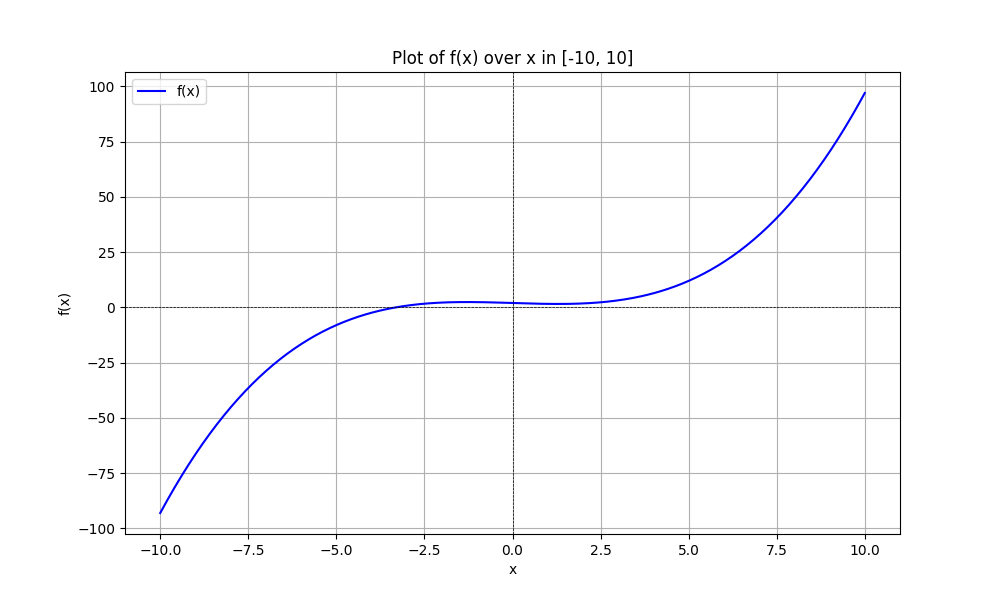
\includegraphics[width=0.6\textwidth]{images/plot1d.png}
\caption{1D plot of a polynomial \( f(x) \) generated by a LangGraph code loop. The agent first created the function definition, verified it, and then produced this plot over the range \( x \in [-10, 10] \).}
\label{fig:langgraph-1d-polynomial}
\end{figure}

%------------------------------------------------------------------------------
%
%------------------------------------------------------------------------------
\subsection*{Visualizing and Interpreting Results}

You can ask the LLM to generate visualization code. We use a second prompt to generate a plot based on the defined function.

\begin{codeonly}{Plotting a Generated Function Using LangChain}
from langchain.prompts import PromptTemplate
from IPython.display import display, Image
from langchain_openai import ChatOpenAI
import os
import traceback

# Initialize model (adjust if already done elsewhere)
llm = ChatOpenAI(model="gpt-4o-mini", temperature=0)

# Prompt to generate a plotting script for f(x)
prompt_plot = PromptTemplate.from_template("""
Given a function f(x) which is defined and you can use - 
do not define f(x) again. Instead, 
write a Python script to plot f(x) over x in [-10, 10] using matplotlib.
Save the figure as 'plot.png'. Return python code only.
""")

# Generate response using the new LangChain syntax
response = (prompt_plot | llm).invoke({})

# Extract the content string from the AIMessage
raw_content2 = response.content.strip()

# Parse out code from markdown fences if needed
if "```python" in raw_content2:
    code_lines2 = raw_content2.split("```python")[1].split("```")[0]
elif "```" in raw_content2:
    code_lines2 = raw_content2.split("```")[1]
else:
    code_lines2 = raw_content2  # fallback

# Save code to file
with open("plot_function.py", "w") as f:
    f.write(code_lines2.strip())

# Try executing the generated plot code
try:
    # Load the function definition into the global scope
    exec(open("f_function.py").read(), globals())
    exec(open("plot_function.py").read(), globals())
    print("Plot executed successfully.")
except Exception:
    print("Error during execution:")
    print(traceback.format_exc())
\end{codeonly}


%------------------------------------------------------------------------------
%
%------------------------------------------------------------------------------
We can also get much more out of the function easily. 

\begin{codeonly}{Interpretation}
prompt_summary = PromptTemplate.from_template(
    "Given the following Python function definition:\n\n{code}\n\n"
    "Describe the mathematical properties of this function (degree, max, min, monotonicity)."
)

chain_summary = prompt_summary | llm
summary = chain_summary.invoke({"code": code_func.content})

from IPython.display import Markdown, display

# Print the function summary as Markdown
print("Function Summary:\n")
display(Markdown(summary.content))
\end{codeonly}

Output is given e.g. by: 

{\footnotesize
\begin{lstlisting}
The function defined in the code is:

[ f(x) = 0.1x^3 - 0.5x + 2 ]

Mathematical Properties:
Degree:

The function is a polynomial of degree 3, as the highest power of (x) is 3.
Maxima and Minima:

To find the local maxima and minima, we need to compute the first derivative of the function and set it to zero: [ f'(x) = \frac{d}{dx}(0.1x^3 - 0.5x + 2) = 0.3x^2 - 0.5 ]
Setting the first derivative to zero: [ 0.3x^2 - 0.5 = 0 \implies 0.3x^2 = 0.5 \implies x^2 = \frac{0.5}{0.3} \implies x^2 = \frac{5}{3} \implies x = \pm \sqrt{\frac{5}{3}} \approx \pm 1.29 ]
To determine whether these points are maxima or minima, we can compute the second derivative: [ f''(x) = \frac{d}{dx}(0.3x^2) = 0.6x ]
Evaluating the second derivative at the critical points:
For (x = \sqrt{\frac{5}{3}}): [ f''\left(\sqrt{\frac{5}{3}}\right) = 0.6\sqrt{\frac{5}{3}} > 0 \quad (\text{local minimum}) ]
For (x = -\sqrt{\frac{5}{3}}): [ f''\left(-\sqrt{\frac{5}{3}}\right) = 0.6(-\sqrt{\frac{5}{3}}) < 0 \quad (\text{local maximum}) ]
Monotonicity:

The function is increasing or decreasing based on the sign of the first derivative (f'(x)):
For (x < -\sqrt{\frac{5}{3}}), (f'(x) < 0) (decreasing).
For (-\sqrt{\frac{5}{3}} < x < \sqrt{\frac{5}{3}}), (f'(x) > 0) (increasing).
For (x > \sqrt{\frac{5}{3}}), (f'(x) > 0) (increasing).
Therefore, the function has a local maximum at (x = -\sqrt{\frac{5}{3}}) and a local minimum at (x = \sqrt{\frac{5}{3}}).
Summary:
Degree: 3
Local Maximum: at (x = -\sqrt{\frac{5}{3}})
Local Minimum: at (x = \sqrt{\frac{5}{3}})
Monotonicity: Decreasing for (x < -\sqrt{\frac{5}{3}}), increasing for (-\sqrt{\frac{5}{3}} < x < \sqrt{\frac{5}{3}}), and increasing for (x > \sqrt{\frac{5}{3}}).
\end{lstlisting}
}

%------------------------------------------------------------------------------
%
%------------------------------------------------------------------------------
\begin{figure}[h]
\centering
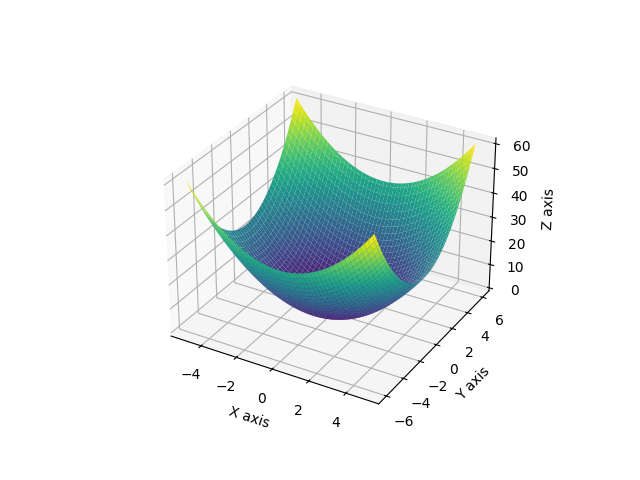
\includegraphics[width=0.75\textwidth]{images/my2d.png}
\caption{2D surface plot of a generated function \( f(x, y) \), created dynamically by a LangGraph agent. The LLM generated the code, saved it, and executed it to render this 3D surface using matplotlib.}
\label{fig:langgraph-2d-function}
\end{figure}

%===============================================================================
%
%===============================================================================
\subsection*{Autonomous Code Execution with a Self-Correcting LLM Loop}

To make our workflow more robust, we wrap the code generation and execution in a loop that automatically retries in case of errors. This allows us to turn LangChain into a simple coding agent that iteratively improves its output.

\begin{codeonly}{Self-Correcting Code Agent Loop}
import traceback

def autonomous_code_agent(prompt, llm, filename="generated_code.py", max_attempts=5):
    from langchain.prompts import PromptTemplate
    from langchain.chains import LLMChain

    template = PromptTemplate.from_template(prompt)
    chain = LLMChain(llm=llm, prompt=template)
    
    current_prompt = ""
    for attempt in range(1, max_attempts + 1):
        print(f"\n=== Attempt {attempt} ===")
        result = chain.invoke({"input": current_prompt})
        code = result.content.strip()

        with open(filename, "w") as f:
            f.write(code)

        try:
            print("Executing...")
            exec(open(filename).read())
            print("Success.")
            return code
        except Exception as e:
            error_msg = traceback.format_exc()
            print("Error:\n", error_msg)
            current_prompt += f"\n\nThe last attempt failed with this error:\n{error_msg}\nPlease fix it and regenerate working Python code."
    
    print("Failed after max attempts.")
    return None
\end{codeonly}

\begin{codeonly}{Running the Code Agent to Create a Function}
prompt_func = (
    "Write a Python function f(x) using numpy that defines a polynomial. "
    "Ensure that |f(x)| stays below 10 for x in [-10, 10]. Name the function f."
)

code = autonomous_code_agent(prompt_func, llm, filename="f_function.py")
\end{codeonly}

\begin{codeonly}{Sanity Check: Test the Function}
exec(open("f_function.py").read())

import numpy as np
print("f(0) =", f(0))
print("f(5) =", f(5))
\end{codeonly}

You can repeat this approach with other tasks, such as plotting or file processing. This pattern is a simple example of a structured LLM agent loop that improves iteratively.


%------------------------------------------------------------------------------
%
%------------------------------------------------------------------------------
\subsection*{Conclusion: LangChain as a Structured Agent Layer}

LangChain provides modular tools to build LLM-powered agents that mix language understanding with logic, plotting, and tool use. In contrast to direct API calls, it helps manage prompt templates, execution chains, and debugging more systematically.


%===============================================================================
%
%===============================================================================
\section{LangGraph-Based Forecast Assistant}

In this section, we demonstrate how LangGraph can be used to build an intelligent assistant that interprets user input, extracts weather-related information (like temperature forecasts), downloads data from official sources, and generates plots or numerical results. This is part of a broader approach combining Large Language Models (LLMs) with structured tool execution.

LangGraph is a library that enables graph-based control flow for LLM applications. Each node in the graph represents a computational or reasoning step, while the edges define the order in which steps are executed. State is passed and updated along the way.

%------------------------------------------------------------------------------
%
%------------------------------------------------------------------------------
\begin{figure}[htbp]
	\centering
	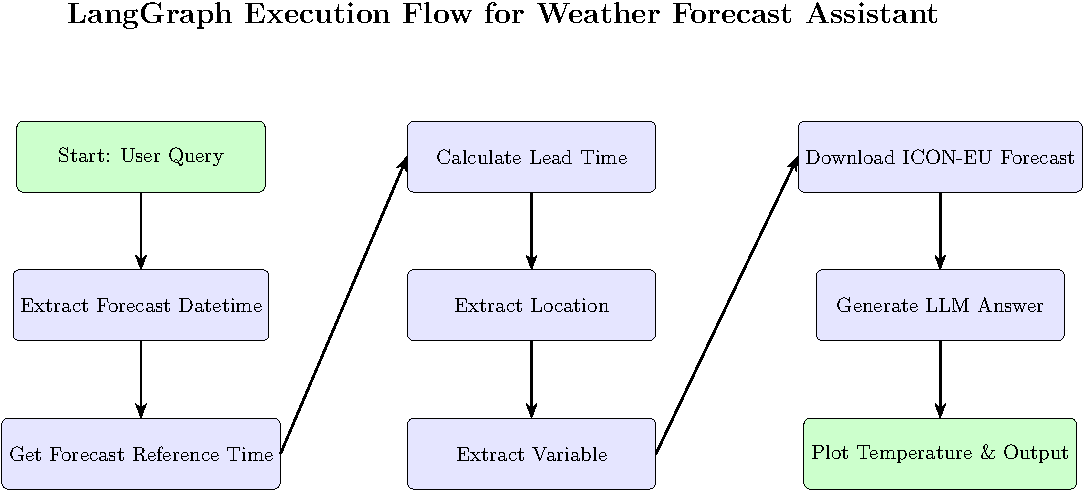
\includegraphics[width=0.9\textwidth]{images/langgraph_weatherforecast2.pdf}
	\caption{Execution flow of the LangGraph-based weather forecast assistant. Each node represents a processing step, starting from the natural language query down to data download and result output.}
	\label{fig:langgraph-weather}
\end{figure}

%------------------------------------------------------------------------------
%
%------------------------------------------------------------------------------
Our assistant interprets queries like:
\textit{Please give me the temperature forecast for Monday 4pm in Berlin.}
It then carries out the following steps, defined by the langgraph graph as visualized in Figure \ref{fig:langgraph-weather}:

\begin{enumerate}
\item LLM: Extracts the forecast date and time from the text.
\item Fkt: Retrieves the latest forecast reference time from DWD.
\item Fkt: Calculates the lead time in hours.
\item LLM: Extracts the location and variable (e.g., ``temperature'').
\item Fkt: Downloads the corresponding ICON-EU GRIB2 data file.
\item LLM: Generate answer to user.
\item Fkt: Plots the temperature field.
\end{enumerate}

%------------------------------------------------------------------------------
%
%------------------------------------------------------------------------------
\subsection*{LangGraph State Definition}

LangGraph requires an explicit state schema. A state schema defines the structure of the data (or "state") that flows through the graph. Each node in the graph receives the state as input, performs some computation, and returns an updated version of the state. The schema ensures that all nodes have a consistent view of what data is available, what fields are expected, and what can be modified or added during execution. We use Python's \texttt{TypedDict} to define all fields that may be shared or updated between graph steps.

\begin{codeonly}{python}
class MyState(TypedDict):
	query: str
	task: str
	output: str
	fc_datetime: str
	fc_reference_datetime: str
	fc_leadtime: str
	fc_plot_option: str
	fc_location_of_interest: str
	fc_variable: str
	fc_lat: str
	fc_lon: str
	temperature_data: Any
	code_task: str
	code_full: str
	code_output: str
	info_topic: str
\end{codeonly}

%------------------------------------------------------------------------------
%
%------------------------------------------------------------------------------
\subsection*{Step 1: Extracting Forecast Datetime}

We use the OpenAI model or a local llama version to extract a specific forecast time from a natural language query. The current system time is included in the prompt to improve accuracy.

\begin{codeonly}{python}
def extract_forecast_datetime(user_input: str) -> str:
	current_time = datetime.datetime.now().strftime("%Y-%m-%d %H")
	prompt = f"""
	The current time is: {current_time}.
	Extract the date and time mentioned in the following user input 
	in format %Y-%m-%d %H.
	User input: {user_input}
	Forecast datetime:
	"""
	response = llm.invoke(prompt)
	return response.content.strip()
\end{codeonly}

%------------------------------------------------------------------------------
%
%------------------------------------------------------------------------------
\subsection*{Step 2: Calculating Lead Time}

Once we know both the reference time and forecast target time, we calculate the lead time in hours (rounded to nearest 3 hours if needed).

\begin{codeonly}{python}
def calculate_forecast_lead_time(forecast_datetime: str, reference_datetime: str) -> int:
	forecast_time = datetime.datetime.strptime(forecast_datetime, "%Y-%m-%d %H")
	reference_time = datetime.datetime.strptime(reference_datetime, "%Y-%m-%d %H")
	lead_time = (forecast_time - reference_time).total_seconds() / 3600
	return int(lead_time)
\end{codeonly}

%------------------------------------------------------------------------------
%
%------------------------------------------------------------------------------
\subsection*{Step 3: Downloading ICON-EU Data}

We download the GRIB2 forecast file for the corresponding forecast hour. The hour is zero-padded (e.g., ``087'') and matched using a regular expression. Data is decompressed and loaded with \texttt{cfgrib}.

\begin{codeonly}{python}
def download_icon_2m_temperature(fc_leadtime: str = "000") -> xr.DataArray:
	fc_leadtime2 = f"{int(fc_leadtime):03d}"
	url = "https://opendata.dwd.de/weather/nwp/icon-eu/grib/00/t_2m/"
	response = requests.get(url)
	soup = BeautifulSoup(response.text, "lxml")
	pattern = re.compile(rf"icon-eu.*_{fc_leadtime2}_T_2M\.grib2\.bz2")
	for link in soup.find_all("a"):
		if pattern.match(link.get("href")):
			filename = link.get("href")
			break
			bz2_path = "downloads/temp.grib2.bz2"
			grib_path = "downloads/temp.grib2"
			with open(bz2_path, "wb") as f:
			f.write(requests.get(url + filename).content)
			with bz2.open(bz2_path, 'rb') as f_in, open(grib_path, 'wb') as f_out:
			f_out.write(f_in.read())
			ds = xr.open_dataset(grib_path, engine="cfgrib", backend_kwargs={"indexpath": ""})
			return ds["t2m"] - 273.15
\end{codeonly}

%------------------------------------------------------------------------------
%
%------------------------------------------------------------------------------
\subsection*{Step 4: Building the LangGraph}

Each of the above steps becomes a node in our LangGraph. The flow is fully defined with edges and a final step.

{How the Graph Builder Works.}
LangGraph allows developers to define a sequence of processing steps (nodes) and connections (edges) between them in a directed computation graph. This is especially useful when building structured workflows that combine logic, LLMs, and functions.
The key components are:
\begin{itemize}
  \item \textbf{\texttt{builder = create\_graph()}} \\
    Initializes an empty computation graph. This object holds all nodes and edges you define.
    
  \item \textbf{\texttt{builder.add\_node("name", function)}} \\
    Registers a node in the graph with a unique name and an associated callable (e.g., a Python function, LangChain Runnable, or LLM chain). The node will process input and optionally update shared state.

  \item \textbf{\texttt{builder.add\_edge("source", "target")}} \\
    Connects two nodes, specifying that once \texttt{source} finishes execution, its result should be passed to \texttt{target}.
\end{itemize}

During execution, LangGraph processes nodes as follows:

\begin{enumerate}
  \item Starts from the initial node (e.g., \texttt{"start"}).
  \item Passes a shared state (a Python dictionary) from node to node along the defined edges.
  \item Executes the function or LLM associated with each node.
  \item Updates the state with results from each step.
  \item Terminates once a final node is reached or the graph ends.
\end{enumerate}

This mechanism allows combining LLM calls, parsing functions, data downloads, and visualizations into a reproducible and inspectable pipeline.

\begin{codeonly}{python}
# Define the LangGraph schema and state
builder = StateGraph(state_schema=MyState)

# Add nodes (ohne output_keys)
builder.add_node("extract_forecast_datetime", extract_forecast_datetime_node)
builder.add_node("get_latest_forecast_reference_time", get_latest_forecast_reference_time_node)
builder.add_node("calculate_lead_time", calculate_lead_time_node)
builder.add_node("extract_location", extract_location_node)
builder.add_node("extract_variable", extract_variable_node)
builder.add_node("download_temperature", download_temperature_node)
builder.add_node("plot_temperature", plot_temperature_node)
#builder.add_node("get_coordinates", get_coordinates_from_name_node)
#builder.add_node("interpolate_temperature", interpolate_temperature_node)

# Set entry and finish points
builder.set_entry_point("extract_forecast_datetime")
builder.add_edge("extract_forecast_datetime", "get_latest_forecast_reference_time")
builder.add_edge("get_latest_forecast_reference_time", "calculate_lead_time")
builder.add_edge("calculate_lead_time", "extract_location")
builder.add_edge("extract_location", "extract_variable")
builder.add_edge("extract_variable", "download_temperature")
builder.add_edge("download_temperature", "plot_temperature")
#builder.add_edge("download_temperature", "get_coordinates")
#builder.add_edge("get_coordinates", "interpolate_temperature")
builder.set_finish_point("plot_temperature")
#builder.set_finish_point("interpolate_temperature")

# Compile the graph
graph = builder.compile()
\end{codeonly}

%-------------------------------------------------------------------------------
%
%-------------------------------------------------------------------------------
\begin{figure}[htpb]
\centering
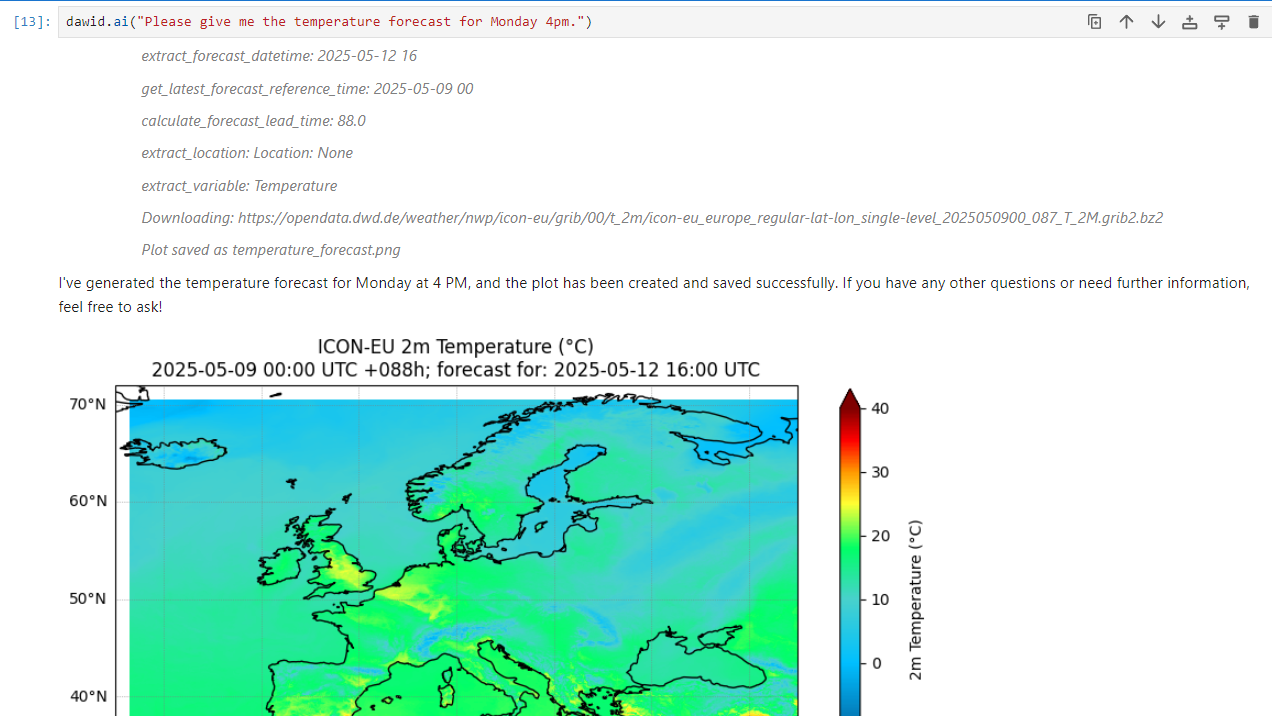
\includegraphics[width=0.99\textwidth]{images/langgraph_weather_forecast.png}
\caption{Weather forecast visualization generated by a LangGraph workflow. The agent pipeline extracted the user's query, downloaded DWD ICON data, interpolated values, and created a temperature map using Cartopy.}
\label{fig:langgraph-weather-forecast}
\end{figure}

%-------------------------------------------------------------------------------
%
%-------------------------------------------------------------------------------
\subsection*{Execution}
The assistant is triggered by calling \texttt{ai(query)}, which sets up the state and runs the graph.

\begin{codeonly}{python}
def ai(query):
    # Initialize state
    state = {
        "query": query,
        "task": "fc",
        "output": "",
        "fc_datetime": "",
        "fc_reference_datetime": "",
        "fc_leadtime": "",
        "fc_plot_option": "full",
        "fc_location_of_interest": "",
        "fc_variable": "",
        "temperature_data": None,
        "code_task": "",
        "code_full": "",
        "code_output": "",
        "info_topic": ""
    }

    # Run the LangGraph
    result = graph.invoke(state)

    # Generate a summary using the LLM
    summary_prompt = f"""
    You are DAWID, the friendly assistant of Deutscher Wetterdienst. The user asked: "{state["query"]}"

    Intermediate results:
    - Forecast datetime: {result['fc_datetime']}
    - Forecast reference: {result['fc_reference_datetime']}
    - Lead time: {result['fc_leadtime']} hours
    - Location: {result['fc_location_of_interest']}
    - Variable: {result['fc_variable']}

    Final output: {result['output']}

    Summarize this in one or two friendly sentences for the user.
    """

    response = llm.invoke(summary_prompt)
    display(Markdown(response.content))
\end{codeonly}

\textbf{Example:}

\begin{codeonly}{python}
	ai("Please give me the temperature forecast for Sunday 4pm in Berlin.")
\end{codeonly}

This triggers all graph nodes in order, downloads and processes the forecast, and finally plots or returns interpolated values.

\bigskip
LangGraph provides an approach to compose toolchains driven by LLMs, where each step is modular, inspectable, and testable — ideal for modular workflows and AI-based assistants.

